\section{PROBLEM FORMULATION}
\label{sec:problemFormulation}
\noindent\uline{Five types of Platonic Solids}: 
\begin{figure}[h]
\centering
	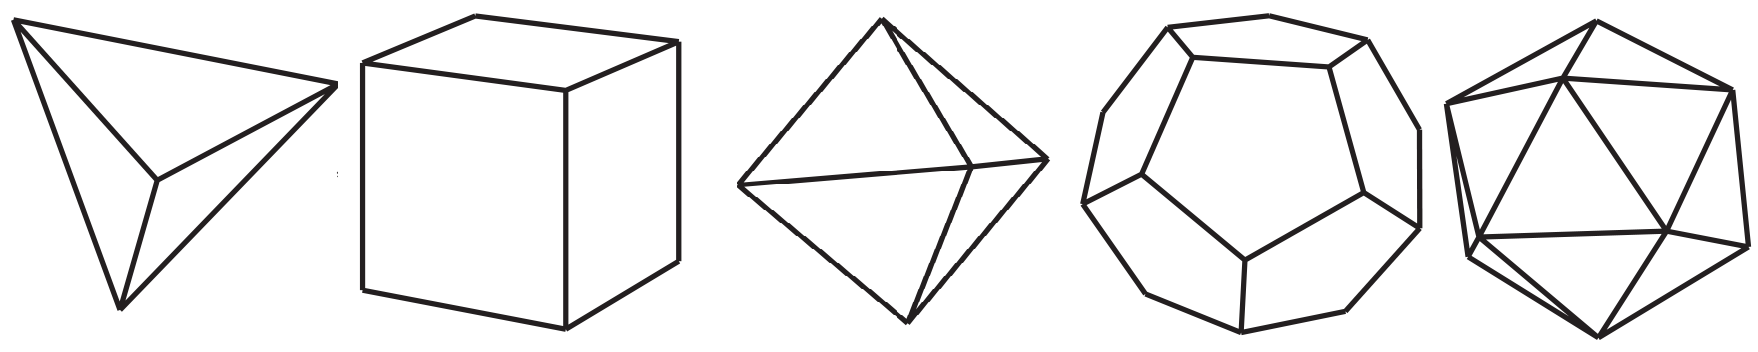
\includegraphics[width=1\textwidth]{image/5Platonic.png}
	\caption{Platonic solids. From left to right: Tetrahedron, Cube, Octahedron, Dodecahedron, and Icosahedron}
	\label{fig:platonicSolids}
\end{figure}
%
% 
%
%
%
%
%
Platonic solids properties:
The platonic solids are also called regular polyhedra have the convex polyhedra properties. There are only five solids namely cube, tetrahedron, octahedron, dodecahedron and icosahedron. Some of the equivalent statements are used to describe the platonic solids including all the vertices lie on a sphere, all the dihedral angle are equal, and all solid angles are equivalent.\\

\noindent Here is your table \ref{tab:tb1}

\begin{table}[h]
\centering
\caption{Properties of polyhedron}
\label{tab:tb1}
\begin{tabular}{|l|c|c|c|c|c|}
\hline
             & Faces & Edges & Vertices & Edges on each face & Edges meeting at each vertices \\ \hline
Tetrahedron  & 4     & 6     & 4        & 3                  & 3                            \\ \hline
Cube         & 6     & 12    & 8        & 4                  & 3                            \\ \hline
Octahedron   & 8     & 12    & 6        & 3                  & 4                            \\ \hline
Dodecahedron & 12    & 30    & 20       & 5                  & 3                            \\ \hline
Icosahedron  & 20    & 30    & 12       & 3                  & 5                            \\ \hline
\end{tabular}
\end{table}
% generate the table from https://www.tablesgenerator.com/#






Here is your table \ref{tab:tb2}

\begin{table}[h]
\centering
\caption{Dimensional of platonic solids}
\label{tab:tb2}
\begin{tabular}{|l|c|c|c|c|}
\hline
             & $r_d$	                             & $\rho$                    & R	     					      & dihedral angles ($\beta$)	\\ \hline
Tetrahedron  & $\frac{1}{12}\sqrt{6}$    			 & $\frac{1}{4}\sqrt{2}$     & $\frac{1}{4}\sqrt{6}$              & $\cos^{-1}(\frac{1}{3})$                       \\ \hline
Cube         & $\frac{1}{2}$                         & $\frac{1}{2}\sqrt{2}$     & $\frac{1}{2}\sqrt{3}$              & $\frac{1}{2}\pi$                \\ \hline
Octahedron   & $\frac{1}{6}\sqrt{6}$    			 & $\frac{1}{2}$    	     & $\frac{1}{2}\sqrt{2}$      		  & $\cos^{-1}(-\frac{1}{3})$               \\ \hline
Dodecahedron & $\frac{1}{20}\sqrt{250+110\sqrt{5}}$  & $\frac{1}{4}(3+\sqrt{5})$ & $\frac{1}{4}(\sqrt{15}+\sqrt{3})$  & $\cos^{-1}(-\frac{1}{5}\sqrt{5})$              \\ \hline
Icosahedron  & $\frac{1}{12}(3\sqrt{3}+\sqrt{15})$   & $\frac{1}{4}(1+\sqrt{5})$  & $\frac{1}{4}\sqrt{10+2\sqrt{5}}$  & $\cos^{-1}(-\frac{1}{3}\sqrt{5})$               \\ \hline
\end{tabular}
\end{table}

\clearpage
\newpage

























%\vspace{1in}
%\begin{table}%[h!]
%	\centering
%	\caption{Optimized Parameter Values}
%	\begin{tabular}{llllp{7em}p{7em}l}
%		\toprule
%		Type of Controller & Parameter    & Xmax & Xmin & \raggedright Iter. reqd. for convergence & Optimized value & $W_\mathrm{min}$ \\ \midrule
%			PSO-SOSMC        & $c_1$        & 5    & 0.1  & 37                                       & 4.75            & 68.43 \\
%			                 & $c_2$        & 5    & 0.1  & 10                                       & 4.273           & 20.45 \\
%			                 & $\lambda_1 $ & 5    & 0.1  & 37                                       & 2.75            & 68.43\\
%			                 & $\lambda_2 $ & 5    & 0.1  & 10                                       & 3.59            & 20.45\\
%			                 & $W_1 $       & 1    & 0.05 & 37                                       & 0.43            & 68.45\\
%			                 & $W_2 $       & 1    & 0.05 & 10                                       & 0.218           & 20.43\\ \cmidrule(lr){2-7}
%			PSO-BELBIC       & $W_1$        & 5    & 0.1  & 36                                       & 4.5             & 27.34 \\
%			                 & $W_2$        & 5    & 0.1  & 14                                       & 4.5             & 61.63 \\
%			                 & $G_1$        & 5    & 0.1  & 36                                       & 1.4             & 27.34 \\
%			                 & $G_2$        & 5    & 0.1  & 14                                       & 1.4             & 61.63\\ \bottomrule
%		\end{tabular}
%\end{table}